\documentclass{article}

\usepackage{arxiv}

\usepackage[utf8]{inputenc} % allow utf-8 input
\usepackage[T1]{fontenc}    % use 8-bit T1 fonts
\usepackage{lmodern}        % https://github.com/rstudio/rticles/issues/343
\usepackage{hyperref}       % hyperlinks
\usepackage{url}            % simple URL typesetting
\usepackage{booktabs}       % professional-quality tables
\usepackage{amsfonts}       % blackboard math symbols
\usepackage{nicefrac}       % compact symbols for 1/2, etc.
\usepackage{microtype}      % microtypography
\usepackage{lipsum}
\usepackage{graphicx}

\title{Accessibility to Primary Care Physicians: Comparing Floating
Catchments with a Utility-based Approach}

\author{
  }


% Pandoc citation processing
\newlength{\csllabelwidth}
\setlength{\csllabelwidth}{3em}
\newlength{\cslhangindent}
\setlength{\cslhangindent}{1.5em}
% for Pandoc 2.8 to 2.10.1
\newenvironment{cslreferences}%
  {}%
  {\par}
% For Pandoc 2.11+
\newenvironment{CSLReferences}[3] % #1 hanging-ident, #2 entry spacing
 {% don't indent paragraphs
  \setlength{\parindent}{0pt}
  % turn on hanging indent if param 1 is 1
  \ifodd #1 \everypar{\setlength{\hangindent}{\cslhangindent}}\ignorespaces\fi
  % set entry spacing
  \ifnum #2 > 0
  \setlength{\parskip}{#2\baselineskip}
  \fi
 }%
 {}
\usepackage{calc} % for calculating minipage widths
\newcommand{\CSLBlock}[1]{#1\hfill\break}
\newcommand{\CSLLeftMargin}[1]{\parbox[t]{\csllabelwidth}{#1}}
\newcommand{\CSLRightInline}[1]{\parbox[t]{\linewidth - \csllabelwidth}{#1}}
\newcommand{\CSLIndent}[1]{\hspace{\cslhangindent}#1}



\begin{document}
\maketitle

\def\tightlist{}


\begin{abstract}
text goes here
\end{abstract}

\keywords{
    accessibility analysis
   \and
    text
   \and
    text
   \and
    text
  }

\hypertarget{introduction}{%
\section{Introduction}\label{introduction}}

The COVID-19 global pandemic has emphasized the importance of healthcare
accessibility, particularly access to primary care physicians, who
provide the first point of contact between patients and the healthcare
system. In Canada, the Canada Health Act states that all residents
should have ``reasonable access'' to healthcare. However, the 2017
Canadian Community Health Survey revealed that 15.3\% of Canadians aged
12 or over did not have a primary care physician, of whom 17.2\% stated
that there is no physician accessible within their area (StatsCan 2019).

Accessibility to healthcare services is defined by both spatial and
aspatial components (Joseph and Bantock 1982). Aspatial factors include
the cost and quality of healthcare services and the socioeconomic,
demographic, and mobility profile of potential users (Joseph and Bantock
1982). The second component considers geographic accessibility, which
can be defined as the potential to interact with a given set of
opportunities, such as healthcare facilities or primary care physicians,
from a given location using the transportation network (Hansen 1959).
Accessibility to healthcare can therefore be improved through either an
increase in the number of available opportunities or through
improvements to the transportation network.

In general, four approaches for calculating accessibility exist:
infrastructure-based approaches, which focus on the capacity of
transportation infrastructure; location-based approaches, which focus on
spatial distributions of opportunities; person-based approaches, which
focus on accessibility on an individual level; and utility-based
measures, which focus on the utility derived from interacting with the
opportunity or participating in an activity (Geurs and van Wee 2004). Of
these, place-based measures are the most common in the literature and,
of these, the family of ``floating catchment area'' (FCA) methods is one
of the most popular approaches for calculating place-based healthcare
accessibility. Because healthcare access is sensitive to demand and
supply, Luo and Wang (Luo and Wang 2003) (drawing on Radke and Mu
(2000)) introduced the Two-step Floating Catchment Area (2SFCA) method
that first estimates the demand for healthcare at service locations from
population zones and then allocates the level of service back to the
population zones using a binary measure of travel impedance.

Since then, various improvements have been made to the 2SFCA approach to
better capture the friction of distance. The original 2SFCA has been
criticized for over-estimating demand and under-estimating levels of
service in the estimation of accessibilities due to the
multiple-counting of populations that arises from the overlapping
catchments in a study area. In response, researchers have proposed
solutions such as the Three-step Floating Catchment Area (3SFCA) (Wan,
Zou, and Sternberg 2012), Modified 2SFCA (M2SFCA) (Delamater 2013), and
Balanced 2SFCA (B2SFCA) (Paez, Higgins, and Vivona 2019) methods. Of
these, the B2SFCA is the only approach that preserves the original
population and resulting levels of service in calculating floating
catchment accessibilities.

However, despite these innovations, FCA methods remain limited in
several ways. First, FCA approaches often inflate or deflate demand and
supply in the calculation of healthcare access. While the B2SFCA
remedies this, it does so by assigning fractions of populations to
clinics and service ratios to population zones. While the parameters of
the balanced method sum to the original zonal populations and
provider-to-population ratios, this fractional approach does not reflect
the ways in which individuals choose to visit facilities. Second, the
appeal of any given healthcare facility from the perspective of the
population is based solely on its distance or travel time from the
origin zone using the transportation network.

In response, this research utilizes a random utility-based formulation
for modelling accessibility to healthcare services. In contrast to FCA
approaches, each patient is, on average, assigned to a single clinic,
avoiding the issue of double-counting and inflation/deflation of the
demand and levels-of-service respectively in the 2SFCA methods and the
assignment of fractional individuals to clinics in the B2SFCA method.
Beyond travel time, this specification also allows the analyst to
include additional characteristics of the facilities that affect their
appeal, such as CONGESTION. To illustrate the potential of the MNL
approach, we compare it against the use of the 2SFCA and B2SFCA, both
using a continuous decay function.

\hypertarget{methodology}{%
\section{Methodology}\label{methodology}}

\hypertarget{floating-catchment-methods}{%
\subsection{Floating Catchment
Methods}\label{floating-catchment-methods}}

The 2-step floating catchment area (2SFCA) method, developed by Luo and
Wang, calculates accessibility to healthcare using catchment areas based
on a travel time threshold (Luo and Wang 2003). The first step of this
method is calculating the physician-to-population ratio, \(R_j\), for
each clinic at location \(j\):

\[
R_j = \frac{S_j}{\sum_i{P_iW_{ij}}}
\]

Where \(S_j\) is the number of physicians at clinic \(j\) and \(P_i\) is
the population of zone \(i\) weighted by some function of the travel
time \(W_{ij}\) between zones \(i\) and \(j\). In the original 2SFCA,
Luo and Wang (2003) utilize a binary impedance function:

\[
W_{ij} = f(t_{ij}) = \left\{
        \begin{array}{ll}
            1 & \quad t_{ij} \leq t_0 \\
            0 & \quad t_{ij} > t_0
        \end{array}
    \right.
\]

where the weight equals 1 for populations within the travel time
threshold \(t_0\) and zero beyond. In this case, Luo and Wang (2003) set
\(t_0 = 15\) minutes. The second step calculates accessibility \(A_i\)
for the population centres as the sum of the physician-to-population
ratios \(R_j\) weighted by the impedance function:

\[
A_i = \sum_j{R_jW_{ij}}
\]

While the 2SFCA approach is a special case of a gravity-based
accessibility measure, the binary impedance function used by Luo and
Wang (2003) does not consider the effects of competition and travel
impedance within a given catchment area. All clinics within a population
centre's catchment area are considered equally accessible, regardless of
distance, size, wait times, or any other measures of attractiveness.
Moreover, all clinics outside of a population centre's catchment area
are considered completely inaccessible. To remedy this, Luo and Qi
(2009) propose the Enhanced 2-step Floating Catchment Area (E2SFCA)
method that introduces categorical weights for different travel time
thresholds to account for travel impedance. Others have improved on the
2SFCA and E2SFCA by using variable catchment sizes (McGrail and
Humphreys 2009), continuous travel time decay functions (Dai 2010), and
adaptive approaches (Bauer and Groneberg 2016) to better reflect travel
time costs and the greater appeal of more proximate opportunities.

Researchers have also sought to improve the ways in which supply and
demand are modeled in floating catchment approaches. Previous research
has shown that both demand and supply can be inflated/deflated in FCA
methods (Delamater 2013; Paez, Higgins, and Vivona 2019; Wan, Zou, and
Sternberg 2012). This is a consequence of the overlapping floating
catchments that cause the populations in zones \(i\) to be counted
multiple times in the calculation of the provider-to-population ratio
\(R_j\). These levels-of-service are, in turn, counted multiple times
when allocated back to the population zones in the calculation of
\(A_i\). In response, Wan et al.~propose the use of additional Gaussian
weights to modify the binary impedance function used by Luo and Wang
(2003). Delamater's (2013) M2SFCA modifies the second step of the 2SFCA
approach by squaring the impedance function to increase the rate of
decay on the level of service. This is done to reflect the increased
friction population centres may experience when accessing healthcare
facilities in sub-optimally configured urban systems.

However, neither of these approaches fully resolves the issue of demand
and supply inflation/deflation. To that end, the B2SFCA approach from
Páez et al. (2019) that replaces the impedance functions with
row-standardized weights \(W_{ij}^{i}\) in the first step:

\[
R_j = \frac{S_j}{\sum_i{P_iW_{ij}^{i}}}
\] \[
W_{ij}^{i} = \frac{W_{ij}}{\sum_j W_{ij}}
\]

and with column-standardized weights \(W_{ij}^{j}\) in the second step:

\[
A_i = \sum_j{R_jW_{ij}^{j}}
\] \[
W_{ij}^{j} = \frac{W_{ij}}{\sum_i W_{ij}}
\]

In this formulation, the travel-time weighted populations sum to the
original population values and do not deflate the level-of-service at
the clinics. By extension, the levels of service available at the
population centres are not inflated through multiple counting. For this
research, we employ both the 2SFCA and B2SFCA approaches with a Gaussian
impedance function:

\[
W_{ij} = e^{-\beta t_{ij}}
\]

where \(\beta\) is a parameter that determines the decay of the Gaussian
function and \(t_{ij}\) is the travel time between clinic \(j\) and
population centre \(i\). The \(\beta\) parameter is set to 0.115 so that
the Gaussian weight would be equal to 0.1 at a 20-minute travel time
threshold.

\hypertarget{utility-based-method}{%
\subsection{Utility-based Method}\label{utility-based-method}}

Despite offering balance across both stages of the FCA approach, the
B2SFCA results in fractional apportionment of the population and
levels-of-service between the population zones and clinics. To address
the limitations of existing methods, a novel methodology is developed
which assigns trips from population centres to clinics. The general form
of this function is as follows:

\[
T_{ij} = f(H_i, Z_j, R_j, t_{ij}, \beta)
\]

where:

\begin{itemize}
\tightlist
\item
  \(T_{ij}\) is the number of trips from zone \(i\) to clinic \(j\)
\item
  \(H_i\) is the number of households in zone \(i\)
\item
  \(Z_j\) is the number of doctors at clinic \(j\)
\item
  \(R_j\) is the demand-to-capacity ratio at clinic \(j\) (note this is
  inverted from the physician-to-population ratios used in previous FCA
  approaches)
\item
  \(t_{ij}\) is the travel time between zones \(i\) and \(j\), and
  \(\beta\) is a row vector of parameters to be estimated.
\end{itemize}

To estimate these parameters, information minimization is used as this
approach allows for the least-biased parameter estimation and has been
proven to be identical to utility maximization (Anas 1983). Based on
information minimization theory, the probability that a household in
zone i will visit clinic j can be estimated as follows:

\[
MAX_{T_{ij}} E = -\sum_{j \in J} \sum_{i \in I} T_{ij} log(T_{ij})
\]

Subject to the following constraints:

\[
\sum_{j \in J}T_{ij} = \alpha H_i \forall i \in I 
\] \[
\sum_{i \in I} \sum_{j \in J} T_{ij} t_{ij} = \bar{t}T 
\] \[
\sum_{i \in I} \sum_{j \in J} T_{ij} log(C_j) = \sum_{i \in I} \sum_{j \in J}T_{ij} log \omega Z_j = \bar{C}T 
\] \[
\sum_{i \in I} \sum_{j \in J} T_{ij} R_j = \bar{R}T
\]

where:

\begin{itemize}
\tightlist
\item
  \(I\) is the set of all residential zones
\item
  \(J\) is the set of all clinics
\item
  \(\alpha\) is the average number of visits to the doctor per household
\item
  \(\bar{t}\) is the average observed travel time for home-based trips
  to clinics
\item
  \(T\) is the total number of daily trips to clinics
\item
  \(C_j\) is the nominal service capacity at clinic \(j\)
\item
  \(\omega\) is the average number of patients served by a doctor per
  day
\item
  \(\bar{C}\) is the average observed nominal service capacity
\item
  \(\bar{R}\) is the average observed demand-to-capacity ratio
\item
  \(H\) is the total number of households
\item
  \(Z\) is the total number of primary care physicians
\end{itemize}

The service capacities and demand-to-capacity ratios are calculated as
follows:

\[
C_j = \omega Z_j \\
R_j = \frac{\sum_{i \in I} T_{ij}}{C_j} = \frac{\sum_{i \in I} T_{ij}}{\omega Z_j}
\]

Solving this set of equations yields the following:

\[
T_{ij} = \alpha H_i P_{ij}
\]

This is a singly-constrained gravity model where the probability that a
household in zone \(i\) will visit clinic \(j\) is as follows:

\[
P_{ij} = \frac{e^{\beta_1 t_{ij} + \beta_{K+2} log \omega Z_j + \beta_{K + 3} R_j}}{\sum_j\prime e^{\beta_1 t_{ij}\prime + \beta_{K+2} log \omega Z_j\prime + \beta_{K + 3} R_j\prime}}
\]

\(\beta_1\), \(\beta_{K+2}\), and \(\beta_{K + 3}\) are all parameters
which should be estimated iteratively in order to meet the outlined
constraints. However, due to a lack of observed data on trips to
doctors, these parameters are instead chosen based on the following
considerations:

\begin{itemize}
\item
  -0.05 is in the range of typical auto travel time parameters in GTHA
  logit mode choice models.
\item
  Random utility theory requires \(\beta_{K+2}\) to lie between 0 to 1
  in value. It is set equal to 1 in this case to maximize the
  attractiveness of larger clinics.
\item
  No theory is currently available to guide the choice of the
  \(\beta_{K+3}\) parameter and so -0.5 is chosen as a ``first guess''
  at a parameter value that would produce a reasonable sensitivity to
  clinic over-crowding, but not prevent over-crowding from occurring.
\end{itemize}

These values ensure that increased travel times and demand-to-capacity
ratios reduce the probability that a household in zone \(i\) will visit
clinic \(j\), and increased capacity at clinic \(j\) increases the
probability. As a result, clinics with higher demand and longer travel
times attract fewer trips, and larger clinics attract more trips.

This model is a multinomial logit destination choice model, which
ensures that demand at clinics is not over-estimated, as each patient on
average is assigned to a single clinic and is not double counted, as
with the 2SFCA method. As shown by Anas (1983), multinomial logit models
are equivalent to gravity models. Following Ben-Akiva and Lerman
(Ben-Akiva \& Lerman, 1985), accessibility can be defined within random
utility theory as the expected maximum utility for a trip. For the
multinomial logit model, it can be shown that this is the natural
logarithm of the denominator of the logit model (the so-called
``logsum'' or ``inclusive value'' term), yielding for this model the
following accessibility measure:

\[
a_i = log(\sum_{j\prime} e^{\beta_1 t_{ij}\prime + \beta_{K+2} log \omega Z_j\prime + \beta_{K + 3} R_j\prime})
\]

In order to ensure that \(\bar{R}\) is approximately equal to 1, the
\(\alpha\) and \(\omega\) parameters are assumed to be 0.065 and 22,
respectively. Since \(R_j\) is a function of \(T_{ij}\) and vice-versa,
an iterative approach is taken to estimate the \(R_j\) values. The end
result is an approach that involves location choice modelling by
maximizing utility for patients, with larger clinics attracting more
trips and more congested clinics with longer travel times attracting
fewer trips.

\hypertarget{study-area}{%
\section{Study Area}\label{study-area}}

\begin{figure}
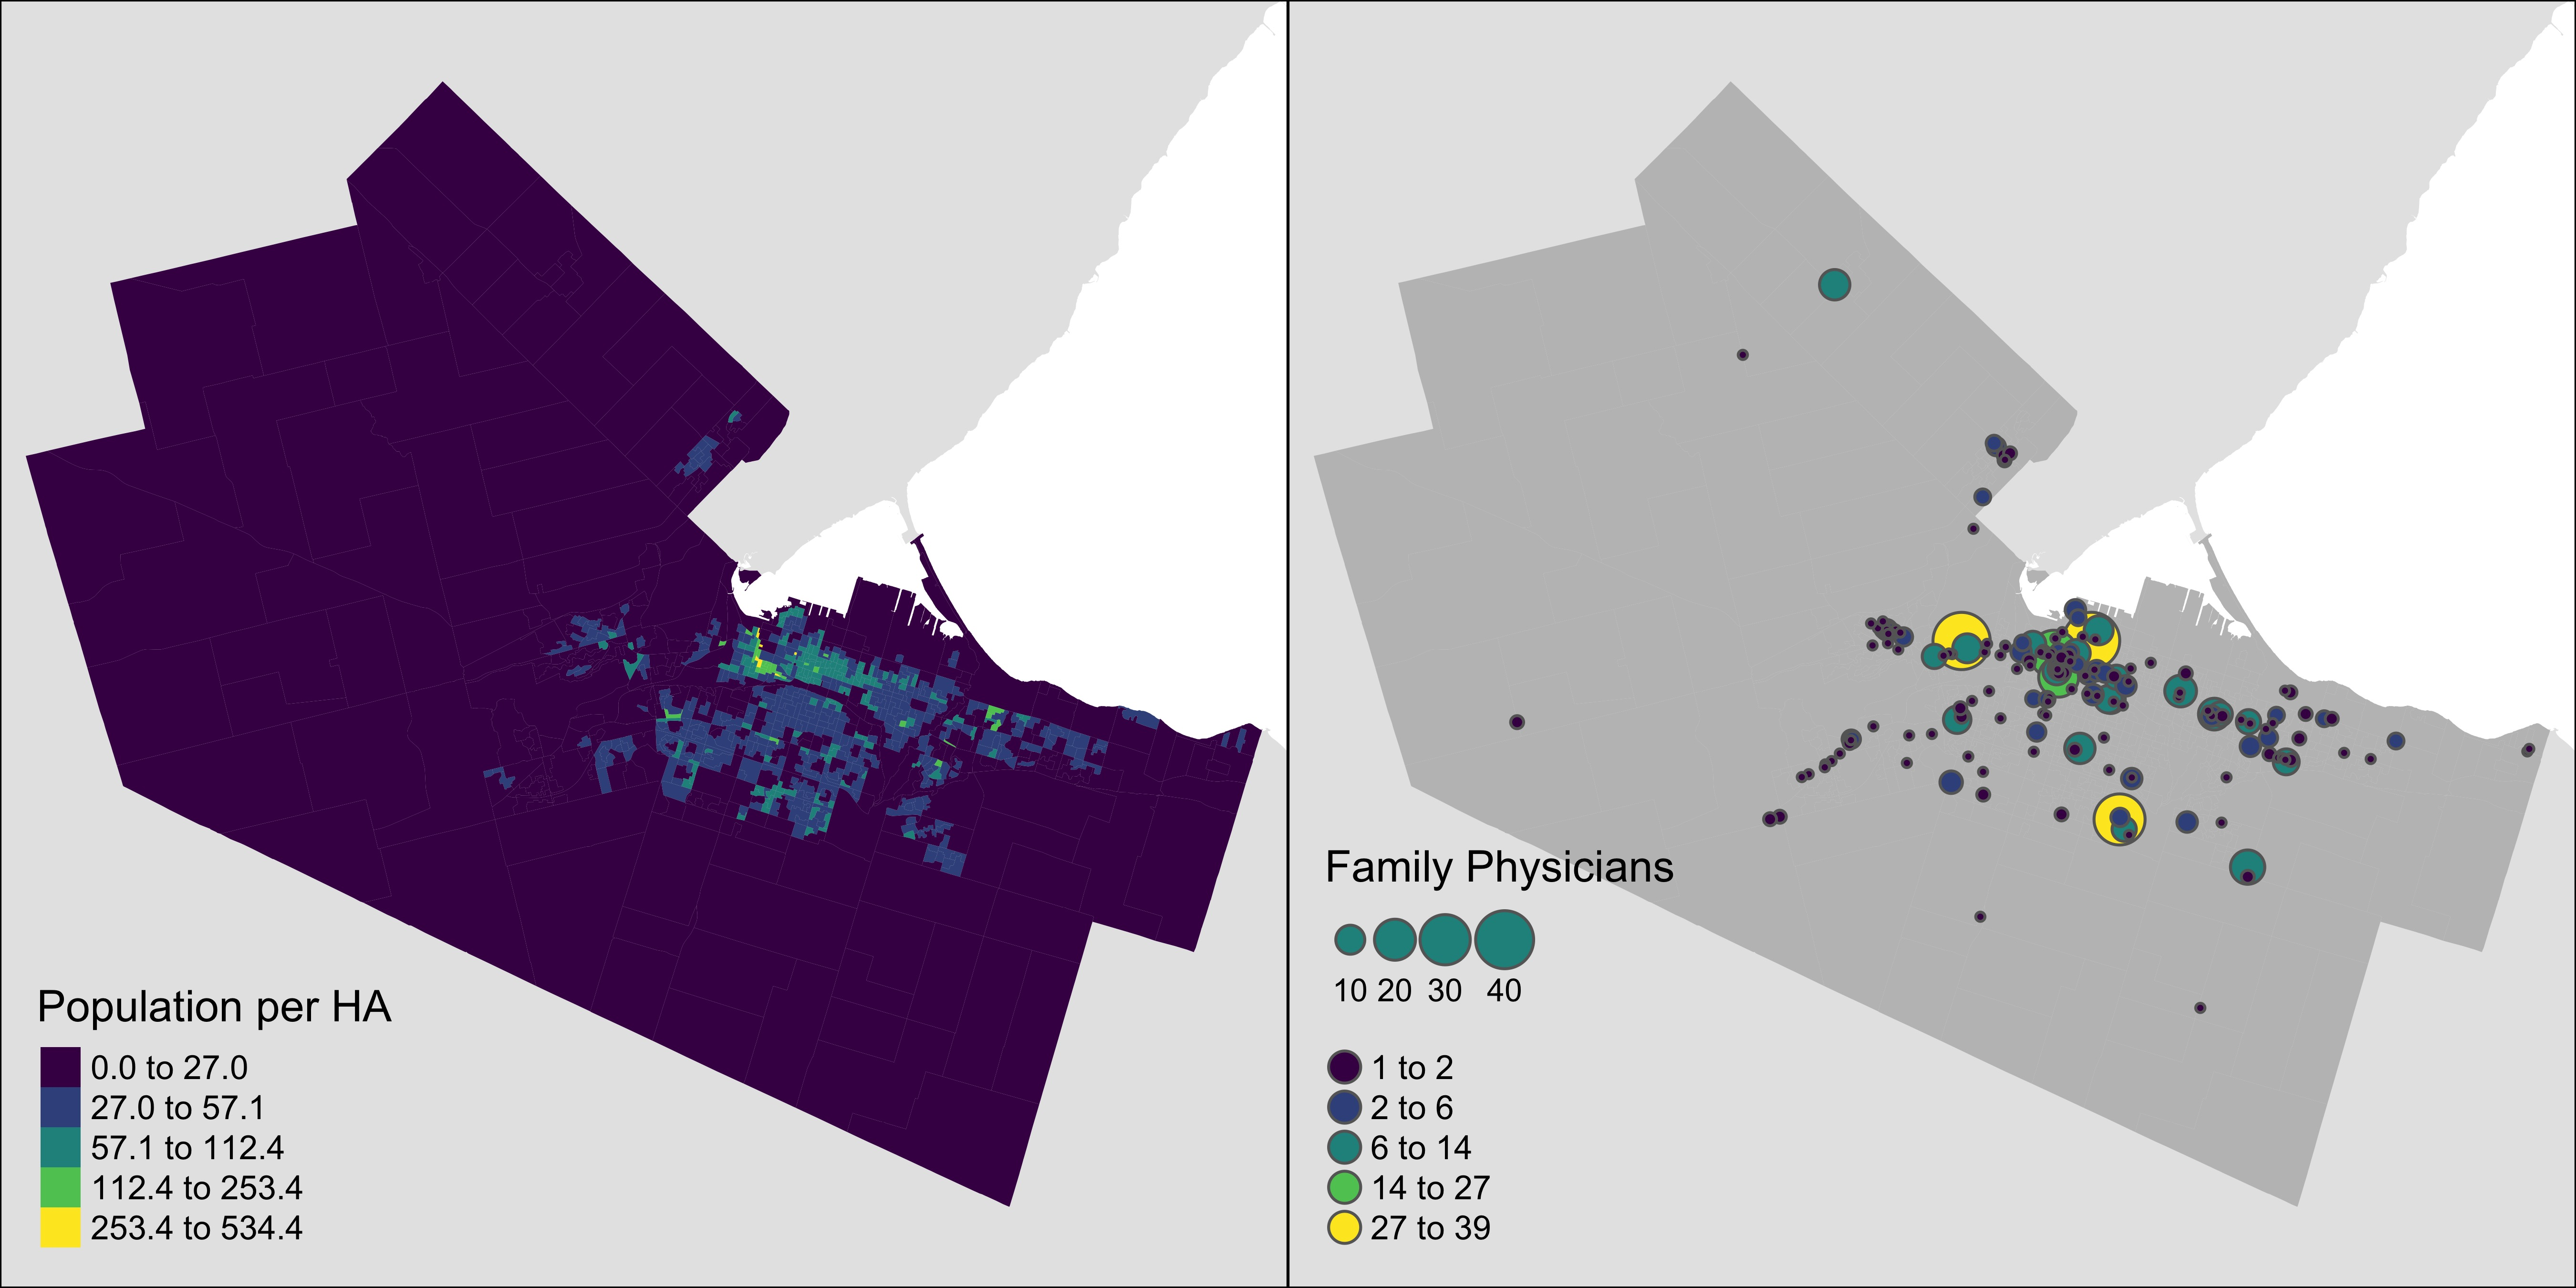
\includegraphics[width=1\linewidth]{./img/Fig_1} \caption{Population Density and Physician Locations}\label{fig:fig 1}
\end{figure}

\hypertarget{results}{%
\section{Results}\label{results}}

\begin{figure}
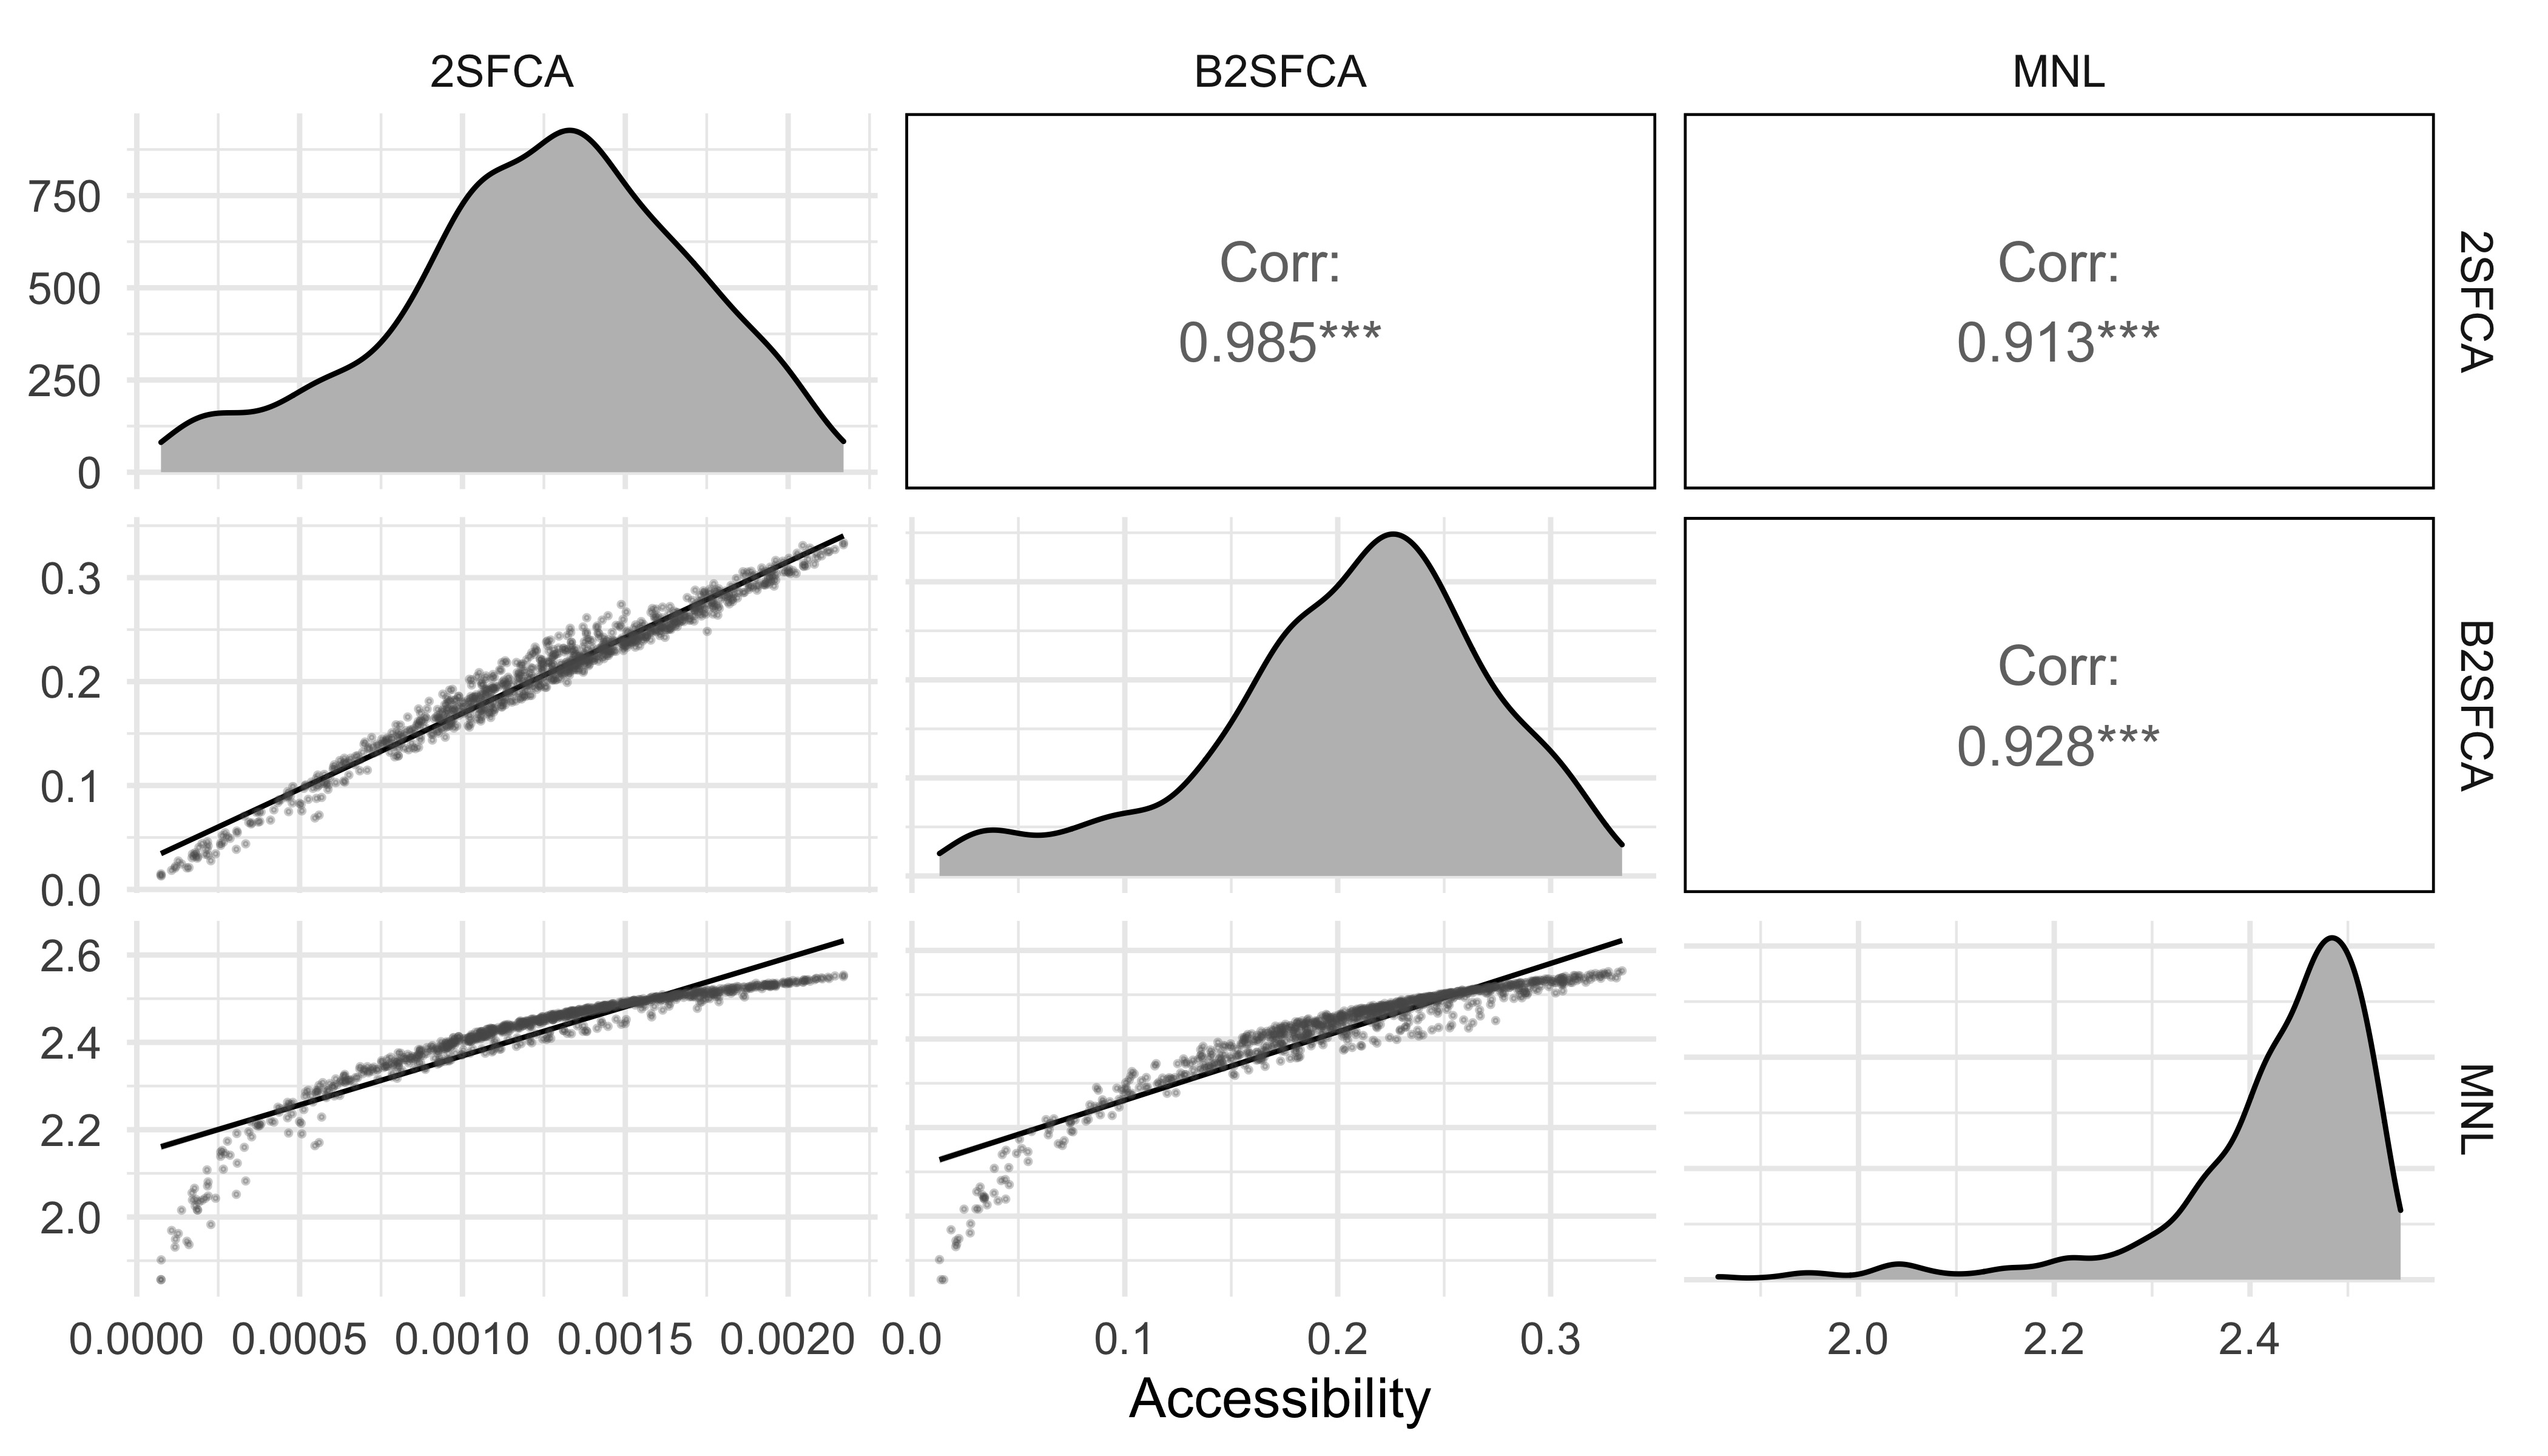
\includegraphics[width=1\linewidth]{./img/Fig_2} \caption{Figure 2. Comparing Distributions}\label{fig:fig 2}
\end{figure}

2SFCA: This pattern indicates that the highest accessibilities to
primary care physicians correspond to the downtown area of Hamilton,
where a large number of clinics are concentrated. Accessibility to
physicians decreases with increased distance from the downtown area. The
distribution of E2SFCA accessibilities to primary care physicians is
presented in XX.

\begin{figure}
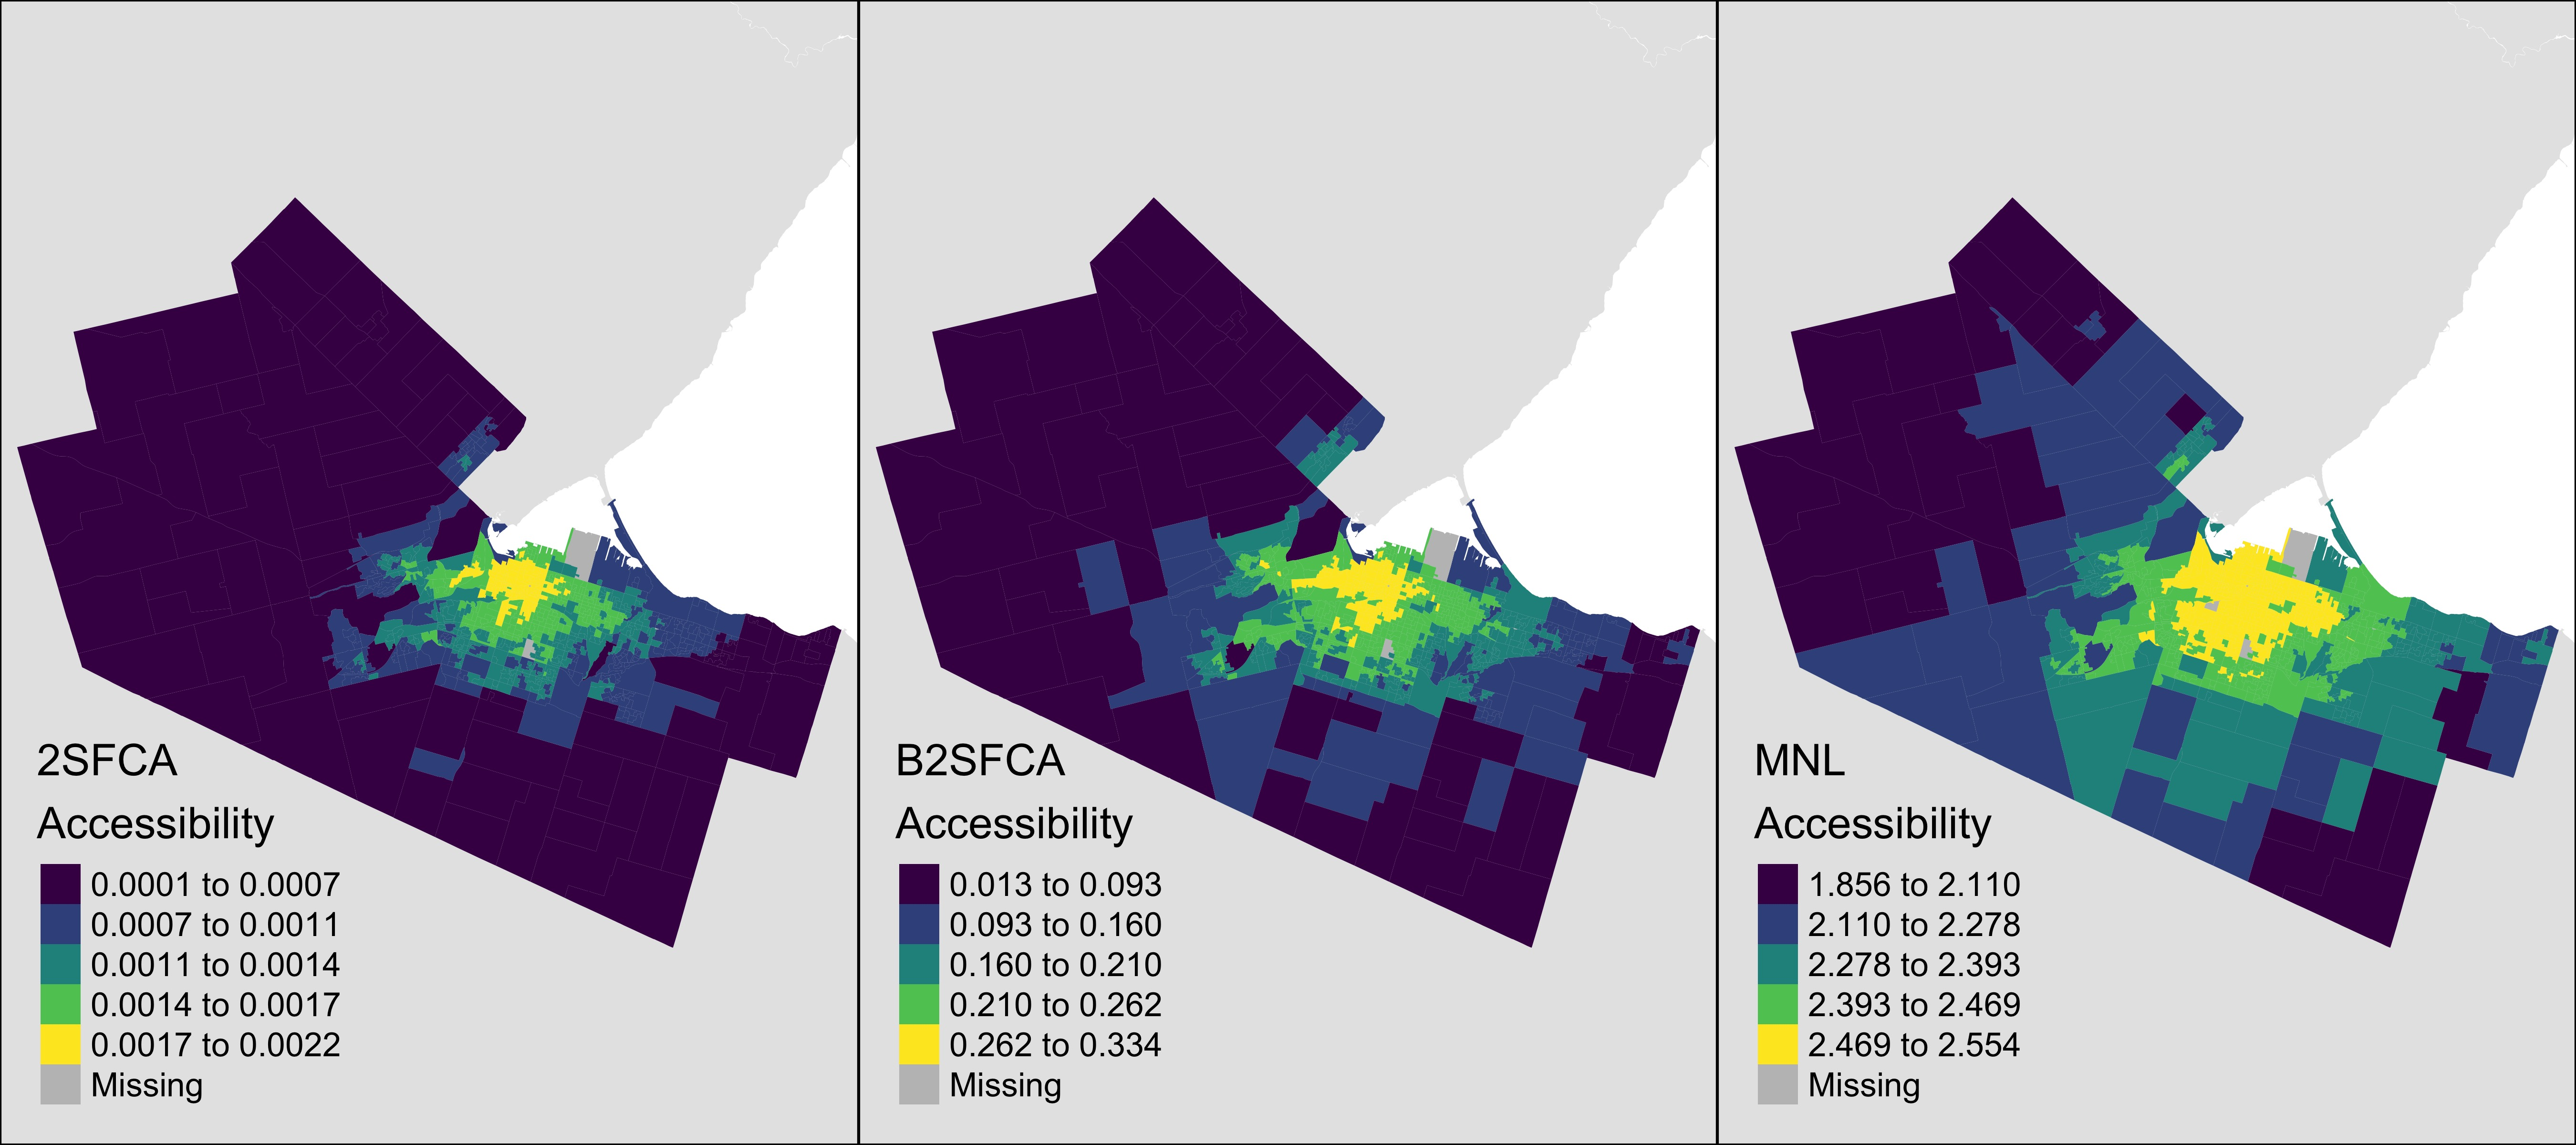
\includegraphics[width=1\linewidth]{./img/Fig_3} \caption{Figure 3. Accessibility Results}\label{fig:fig 3}
\end{figure}

The B2SFCA\ldots{}

MNL: Similar to the pattern produced by the 2SFCA method, this pattern
indicates that the highest accessibilities correspond to the downtown
area and the lowest accessibilities correspond to the outskirts of the
city. However, the area with the highest accessibilities is much larger
with the proposed method, encompassing both the city centre and some
suburban areas. Moreover, the values of the accessibilities are much
higher with the proposed method as compared to the E2SFCA method. This
is due to the difference in the definition of accessibility in both
methods -- the E2SFCA method defines accessibilities based on the
physician-to-population ratios of clinics, resulting in very small
values for accessibility. In contrast, the proposed method defines
accessibilities as the logsum of the multinomial logit model, resulting
in larger values for accessibility. The distribution of accessibilities
to primary care physicians based on the proposed methodology is
presented in XX

\begin{figure}
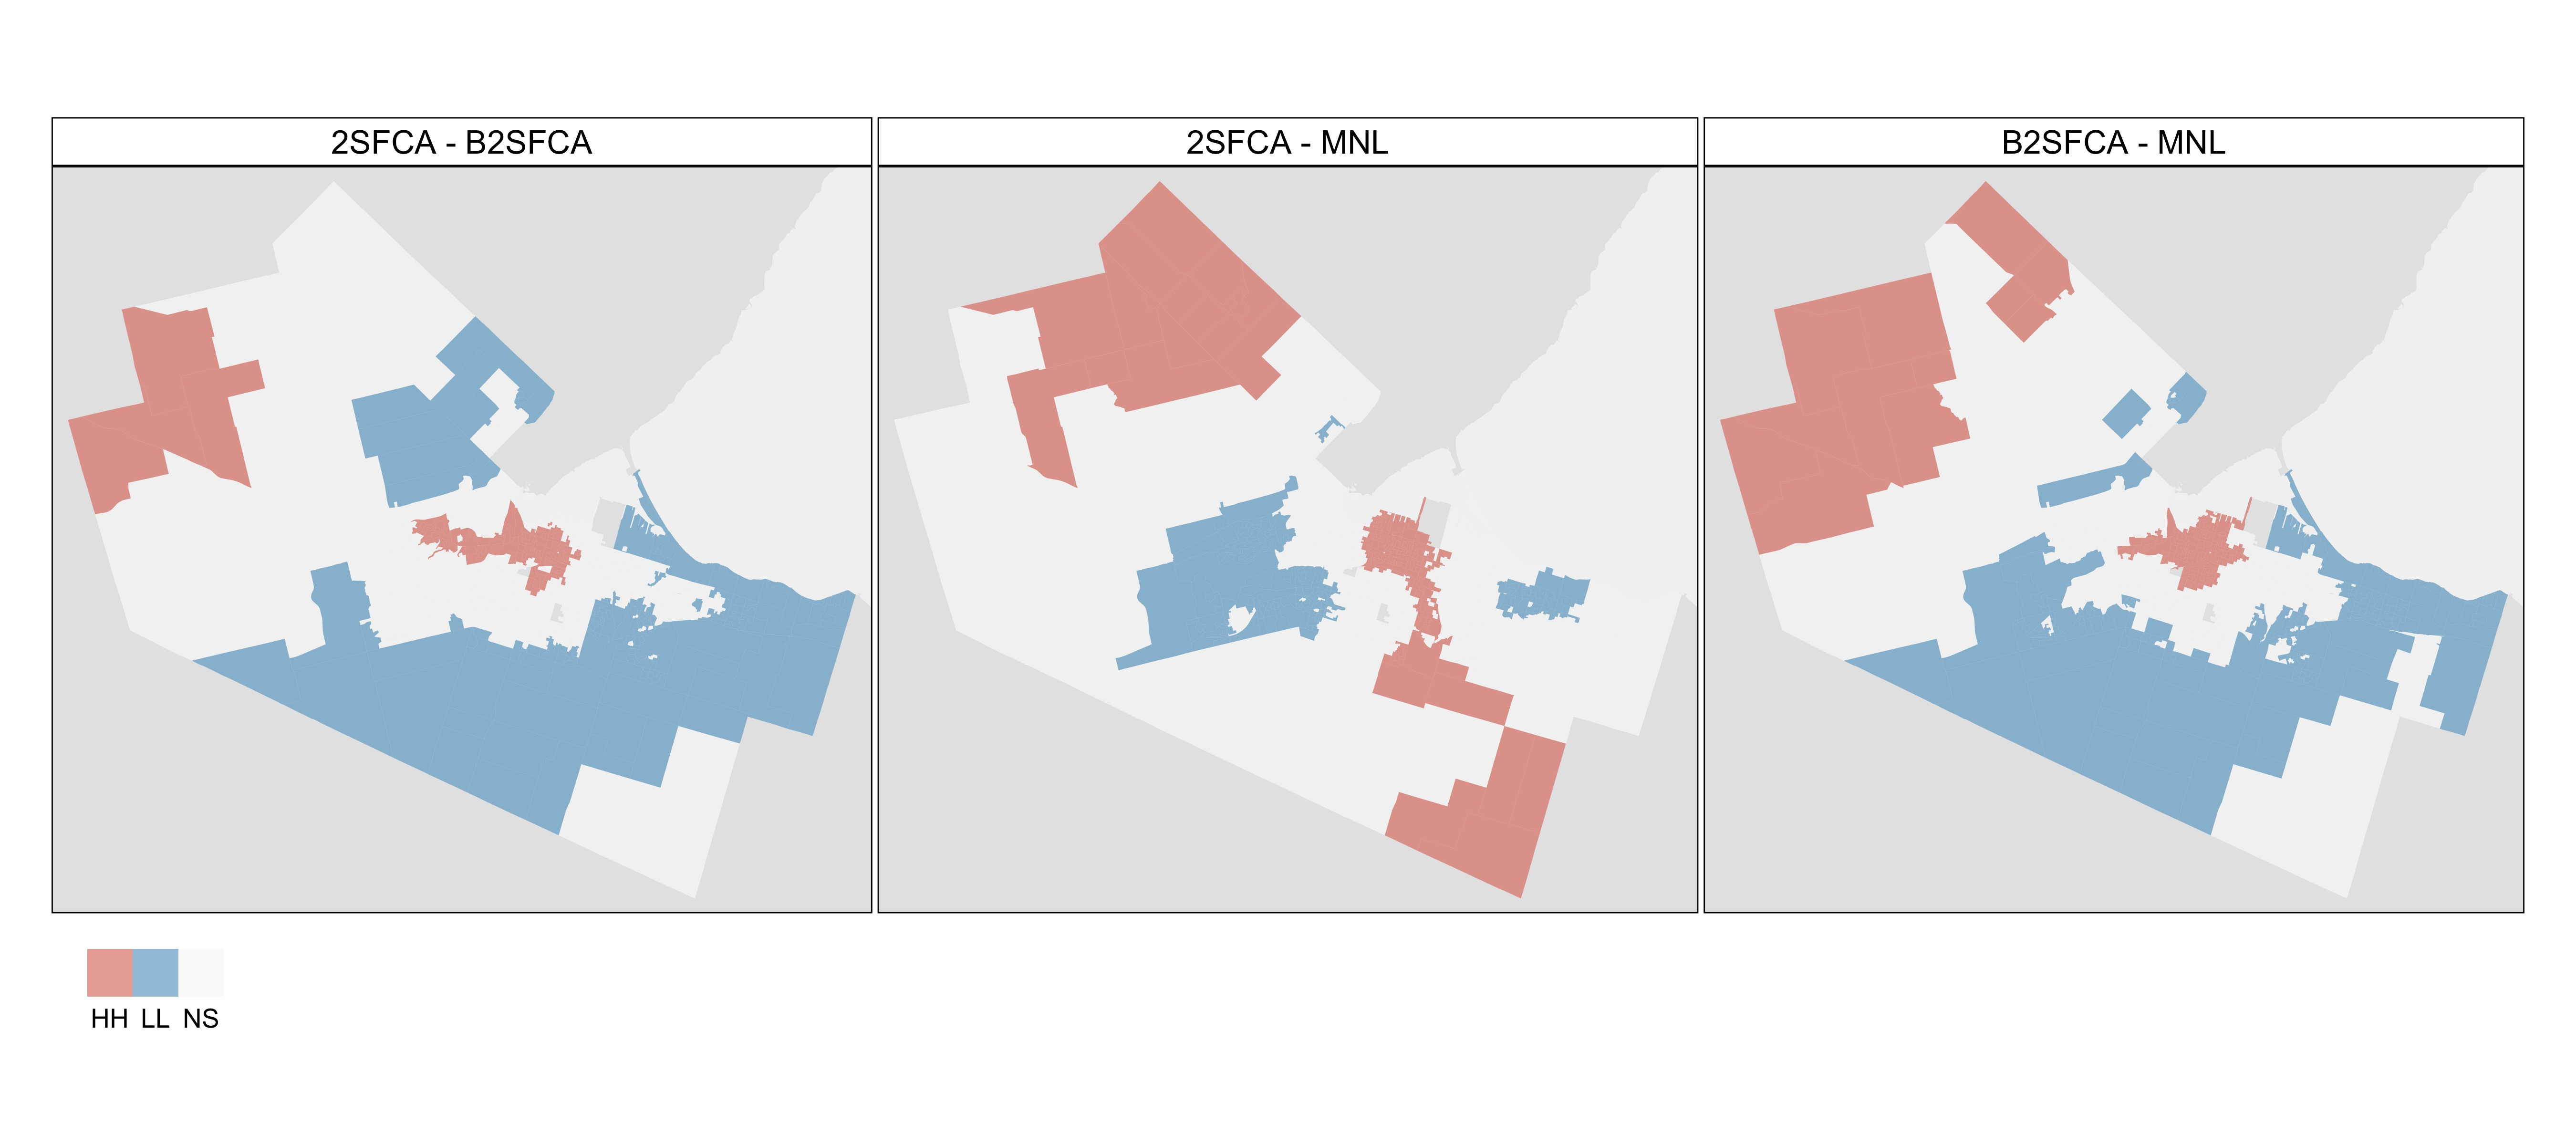
\includegraphics[width=1\linewidth]{./img/Fig_4} \caption{Figure 4. Accessibility Difference Hot Spots}\label{fig:fig 4}
\end{figure}

\hypertarget{discussion-and-conclusions}{%
\section{Discussion and Conclusions}\label{discussion-and-conclusions}}

This study develops a multinomial logit destination choice model for
calculating transportation accessibility to primary care physicians in
the City of Hamilton. This method is compared to the E2SFCA method, and
an analysis of the impact of income on accessibility is undertaken using
both methods. The accessibility patterns produced by both methods
indicate that the highest accessibilities to primary care physicians are
in the downtown area of Hamilton. However, the area with the highest
accessibilities is much larger with the proposed method, encompassing
both the city centre and some suburban areas. The proposed method
produces more plausible distributions as compared to the E2SFCA method,
as more DAs have either medium to high accessibilities or extremely low
accessibilities. In contrast, the E2SFCA method results in many
high-access areas despite congested clinics, as well as low-access areas
with higher accessibilities than the proposed method despite lower
capacities and longer travel times. Overall, the proposed methodology
improves upon existing methods, as it addresses all six of the
accessibility axioms and does not over-estimate demand. Both the E2SFCA
method and the proposed method result in low-income areas having the
highest accessibilities. The sensitivity analysis suggests that
increased development and increased congestion in the City of Hamilton
both result in reduced accessibilities, although the model is more
sensitive to the number of households in comparison to travel times. The
model can therefore be used to project accessibilities in the future and
adjust clinic capacities accordingly. However, more work is required to
calibrate the model to better fit observed data and to include non-auto
modes of travel.

\hypertarget{references}{%
\section*{References}\label{references}}
\addcontentsline{toc}{section}{References}

\hypertarget{refs}{}
\begin{CSLReferences}{1}{0}
\leavevmode\hypertarget{ref-anas1983}{}%
Anas, Alex. 1983. {``Discrete Choice Theory, Information Theory and the
Multinomial Logit and Gravity Models.''} \emph{Transportation Research
Part B: Methodological} 17 (1): 13--23.
\url{https://doi.org/10.1016/0191-2615(83)90023-1}.

\leavevmode\hypertarget{ref-bauer2016}{}%
Bauer, Jan, and David A. Groneberg. 2016. {``Measuring Spatial
Accessibility of Health Care Providers {{}} Introduction of a Variable
Distance Decay Function Within the Floating Catchment Area (FCA)
Method.''} Edited by Kebede Deribe. \emph{PLOS ONE} 11 (7): e0159148.
\url{https://doi.org/10.1371/journal.pone.0159148}.

\leavevmode\hypertarget{ref-dai2010}{}%
Dai, Dajun. 2010. {``Black Residential Segregation, Disparities in
Spatial Access to Health Care Facilities, and Late-Stage Breast Cancer
Diagnosis in Metropolitan Detroit.''} \emph{Health \& Place} 16 (5):
1038--52. \url{https://doi.org/10.1016/j.healthplace.2010.06.012}.

\leavevmode\hypertarget{ref-delamater2013}{}%
Delamater, Paul L. 2013. {``Spatial Accessibility in Suboptimally
Configured Health Care Systems: A Modified Two-Step Floating Catchment
Area (M2sfca) Metric.''} \emph{Health \& Place} 24 (November): 30--43.
\url{https://doi.org/10.1016/j.healthplace.2013.07.012}.

\leavevmode\hypertarget{ref-geurs2004}{}%
Geurs, Karst T., and Bert van Wee. 2004. {``Accessibility Evaluation of
Land-Use and Transport Strategies: Review and Research Directions.''}
\emph{Journal of Transport Geography} 12 (2): 127--40.
\url{https://doi.org/10.1016/j.jtrangeo.2003.10.005}.

\leavevmode\hypertarget{ref-hansen1959}{}%
Hansen, Walter G. 1959. {``How Accessibility Shapes Land Use.''}
\emph{Journal of the American Institute of Planners} 25 (2): 73--76.
\url{https://doi.org/10.1080/01944365908978307}.

\leavevmode\hypertarget{ref-joseph1982}{}%
Joseph, Alun E., and Peter R. Bantock. 1982. {``Measuring Potential
Physical Accessibility to General Practitioners in Rural Areas: A Method
and Case Study.''} \emph{Social Science \& Medicine} 16 (1): 85--90.
\url{https://doi.org/10.1016/0277-9536(82)90428-2}.

\leavevmode\hypertarget{ref-luo2009}{}%
Luo, Wei, and Yi Qi. 2009. {``An Enhanced Two-Step Floating Catchment
Area (E2sfca) Method for Measuring Spatial Accessibility to Primary Care
Physicians.''} \emph{Health \& Place} 15 (4): 1100--1107.
\url{https://doi.org/10.1016/j.healthplace.2009.06.002}.

\leavevmode\hypertarget{ref-luo2003}{}%
Luo, Wei, and Fahui Wang. 2003. {``Measures of Spatial Accessibility to
Health Care in a GIS Environment: Synthesis and a Case Study in the
Chicago Region.''} \emph{Environment and Planning B: Planning and
Design} 30 (6): 865--84. \url{https://doi.org/10.1068/b29120}.

\leavevmode\hypertarget{ref-mcgrail2009}{}%
McGrail, Matthew R., and John S. Humphreys. 2009. {``Measuring Spatial
Accessibility to Primary Care in Rural Areas: Improving the
Effectiveness of the Two-Step Floating Catchment Area Method.''}
\emph{Applied Geography} 29 (4): 533--41.
\url{https://doi.org/10.1016/j.apgeog.2008.12.003}.

\leavevmode\hypertarget{ref-paez2019}{}%
Paez, Antonio, Christopher D. Higgins, and Salvatore F. Vivona. 2019.
{``Demand and Level of Service Inflation in Floating Catchment Area
(FCA) Methods.''} Edited by Tayyab Ikram Shah. \emph{PLOS ONE} 14 (6):
e0218773. \url{https://doi.org/10.1371/journal.pone.0218773}.

\leavevmode\hypertarget{ref-radke2000}{}%
Radke, John, and Lan Mu. 2000. {``Spatial Decompositions, Modeling and
Mapping Service Regions to Predict Access to Social Programs.''}
\emph{Annals of GIS} 6 (2): 105--12.
\url{https://doi.org/10.1080/10824000009480538}.

\leavevmode\hypertarget{ref-statcan2019}{}%
StatsCan. 2019. {``Primary Health Care Providers, 2017.''} Statistics
Canada.

\leavevmode\hypertarget{ref-wan2012}{}%
Wan, Neng, Bin Zou, and Troy Sternberg. 2012. {``A Three-Step Floating
Catchment Area Method for Analyzing Spatial Access to Health
Services.''} \emph{International Journal of Geographical Information
Science} 26 (6): 1073--89.
\url{https://doi.org/10.1080/13658816.2011.624987}.

\end{CSLReferences}

\bibliographystyle{unsrt}
\bibliography{references.bib}


\end{document}
